%\begin{figure}[H]
%    \centering
    \begin{tikzpicture}
        \pgfplotsset{
            width=1.0\textwidth,
            height=0.33\textheight
        }
        \begin{axis}
            [
                xbar=2pt,
                legend style={at={(0.5,-0.18)}, anchor=north,legend columns=-1},
                bar width = 5pt,
                xlabel= DEC (Joules),
                ylabel= Core,
                xmin=0,xmax=90,
                    ytick={0,1,2,3,4,5,6,7},
            ]
            \addplot coordinates { 
                (51.5,0)
                (61.7,1)
                (45.0,2)
                (44.9,3)
                (44.9,4)
                (44.9,5)
                (44.8,6)
                (44.9,7)
                };
            \addplot coordinates { 
                (77.7,0)
                (79.2,1)
                (78.7,2)
                (79.09,3)
                (78.7,4)
                (77.6,5)
                (78.5,6)
                (83.3,7)
                };
            \legend{NB, SN}
            \end{axis}
        \end{tikzpicture}
    % \caption{The DEC for DUT 1, where both benchmarks are compiled on oneAPI}
    \caption{DEC}
%\end{figure}
